\documentclass{beamer}
\usepackage[spanish]{babel}
\usepackage[latin1]{inputenc}
\usepackage{multicol} % indice en 2 columnas
\usepackage{centernot}
\usepackage{amsmath}% http://ctan.org/pkg/amsmath

\newcommand{\notimplies}{%
  \mathrel{{\ooalign{\hidewidth$\not\phantom{=}$\hidewidth\cr$\implies$}}}}


\usetheme{Warsaw}
%\usecolortheme{crane}
\useoutertheme{shadow}
\useinnertheme{rectangles}

\setbeamertemplate{navigation symbols}{} % quitar simbolitos

\title[Tema 5 - Diagonalizaci\'on de endomorfismos]{Diagonalizaci\'on de endomorfismos}
\subtitle{Estudios de Ingenier\'ia}
\author[https://frogames.es]{
Juan Gabriel Gomila%$^{1}$  \and E. Eva$^{2}$ \and S. Serpiente$^{3}$
}
\institute[Frogames]{
 % $^{1-2}$
 Frogames
   \and
  \texttt{https://frogames.es}
}
\date{\today}

\AtBeginSection{
\begin{frame}
  \begin{multicols}{2}
  \tableofcontents[currentsection]   
\end{multicols}
\end{frame}
}

\AtBeginSubsection{
\begin{frame}
  \begin{multicols}{2}
  \tableofcontents[currentsection,currentsubsection]
\end{multicols}
\end{frame}
}



%empieza aqui


\begin{document} 

\frame{\titlepage}

\begin{frame}
  \frametitle{\'Indice}
  \tableofcontents
\end{frame}

\section{Introducci\'on}

\begin{frame}
\frametitle{Introducci\'on}
Antes de entrar matem\'aticamente en el tema de la diagonalizaci\'on de matrices cuadradas, se expondr\'an algunas de las aplicaciones que tienen las matrices diagonales.


Recu\'erdese que una matriz diagonal es una matriz cuadrada que tiene ceros en todos los elementos fuera de su diagonal principal.
\end{frame}

\begin{frame}
\frametitle{Introducci\'on}
La factoritzaci\'on de una matriz dada $A$ en funci\'on de otra matriz diagonal $D$ permite resolver problemas de an\'alisis y estudio de los sistemas el\'ectricos, vibraciones, econom\'ia, etc\'etera, que suelen venir modelizados por ecuaciones diferenciales y en derivadas parciales.


En esta factorizaci\'on juegan un papel muy importante unos escalares denominados \textbf{valores propios} y unos tipos especiales de vectores denominados \textbf{vectores propios}
\end{frame}

\begin{frame}
\frametitle{Introducci\'on}
Un tipo de aplicaci\'on de la diagonalizaci\'on de matrices se encuentra en el an\'alisis de la soluci\'on de un sistema din\'amico a lo largo del tiempo.

Un sistema se caracteriza por el estado de un conjunto de $n$ variables que lo determinan. Este conjunto se puede expresar como un vector de $\mathbb R^n$ las componentes del cual expresan los valores de estas variables
\[(x_1,x_2,\cdots, x_n)\]
Si el estado evoluciona a lo largo del tiempo modificando su valor a cada periodo (cada hora, d\'ia, mes,...) es muy com\'un que la relaci\'on entre los estados del sistema se presenten de forma recursiva:
\end{frame}
 
 
 
\begin{frame}
\frametitle{Introducci\'on}
\begin{itemize}
\item $X_{p+1} = A\cdot X_p$, donde $A$ es una matriz cuadrada de orden $n$
\item$X_p$ representa el estado del sistema en el periodo $p$
\item $X_{p+1}$ representa el estado del sistema en el periodo siguiente $p+1$
\end{itemize}
Entonces, basta con conocer el estado en el periodo inicial $X_0$ (estado inicial del sistema) para poder calcular el estado del sistema en cualquier periodo.

\end{frame}

\begin{frame}
\frametitle{Introducci\'on}
En efecto, si se conoce el estado inicial $X_0$, se puede conocer:
\[X_1 = A\cdot X_0\]
\[X_2 = A\cdot X_1 = A\cdot (A\cdot X_0) = A^2\cdot X_0\]
\[\cdots\]
\[X_m = A^m \cdot X_0\]

Por tanto, para conocer el estado del sistema en el periodo $m$ es necesario el c\'alculo de la matriz $A^m$. Este c\'alculo, como ya se habr\'a imaginado, es bastante complicado y es dif\'icil no equivocarse. En cambio se simplifica bastante en el caso de que $A$ sea diagonalizable (como se recordar\'a del Tema 1 de matrices). 
\end{frame}

\section{Diagonalizaci\'on}

\begin{frame}
\frametitle{Matrices semejantes}
\begin{block}{Matrices semejantes}
Dos matrices $A$ y $A'$ son \textbf{semejantes} si existe una matriz $P$ cuadrada invertible (con $|P|\neq 0$) tal que $A' = P^{-1}\cdot A\cdot P$
\end{block}
\end{frame}

\begin{frame}
\frametitle{Matrices semejantes}
Pi\'ensese que todas las matrices semejantes constituyen las diversas representaciones anal\'iticas de un mismo endomorfismo $f$ de un espacio vectorial $E$ de dimensi\'on $n$ en diferentes bases de $E$.
\begin{figure}[h]
\label{diag}
\centering
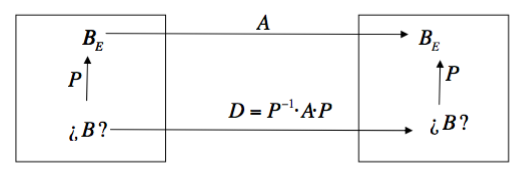
\includegraphics[height=3cm]{im/diagonalitzacio.png}
\end{figure}
\end{frame}

\begin{frame}
\frametitle{Matrices semejantes}
As\'i se plantea el problema de buscar la base de $E$ en la cual $f$ se presenta de la forma m\'as sencilla posible. Debido a las caracter\'isticas tan buenas que presentan las matrices diagonales, se intenta encontrar una base de $E$ en la cual $f$ est\'e representada por una matriz diagonal, es decir, dada una matriz $A$ en una base cualquiera, se va a buscar una matriz diagonal semejante a ella. 

Este proceso recibir\'a el nombre de \textbf{diagonalizar la matriz o el endomorfismo}. 
\end{frame}


\begin{frame}
\frametitle{Matrices diagonalizables}
\begin{block}{Matriz diagonalizable}
Una matriz $A$ es diagonalizable si es semejante a una matriz $D$; es decir, si existe una matriz $P$ regular tal que $D=P^{-1}\cdot A \cdot P$.

No siempre es posible. Habr\'a que estudiar en qu\'e condiciones existe una matriz as\'i y respecto de qu\'e base representar\'a el endomorfismo.
\end{block}
\end{frame}


\section{Vectores y valores propios de una matriz}

\subsection{Definiciones}
\begin{frame}
\frametitle{Matrices diagonalizables}
La teor\'ia que se ver\'a a continuaci\'on est\'a pensada para conseguir llegar a diagonalizar una matriz, pero no se ha de olvidar que esta matriz realmente representa un cierto endomorfismo en una determinada base.
\end{frame}

\begin{frame}
\frametitle{Vectores propios}
\begin{block}{Vector propio (o autovector)}
Dada una matriz cuadrada $A\in M_{n\times n}$ de tama\~no $n$ los vectores columnas de la cual pertenecen a un espacio vectorial $E$ de dimensi\'on $n$, un elemento $\vec x \in E$ es un \textbf{vector propio} de $A$ si:
\begin{enumerate}
\item $\vec x \neq \vec 0$ no es el vector nulo
\item Existe un escalar $\lambda \in \mathbb R$ tal que verifica $A\cdot \vec x = \lambda \vec x$
\end{enumerate}
\end{block}

Geom\'etricamente, un vector propio $\vec x$ es aquel que tiene la mismas direcci\'on que el vector $A\cdot \vec x$ transformado por la matriz $A$. 
\end{frame}

\begin{frame}
\frametitle{Vectorer propios}
\begin{block}{Ejercicio 1}
Demu\'estrese que $\vec x = (2,-1)$ es un vector propio de la matriz $B=\left(\begin{array}{rr}4 & 4 \\1 & 4\end{array}\right)$.
\end{block}
Resulta que $\vec x$ ser\'a un vector propio de la matriz si se cumple que $B\cdot \vec x = \lambda \vec x$ para alg\'un escalar $\lambda$.

\[\left(\begin{array}{rr}4 & 4 \\1 & 4\end{array}\right) \left(\begin{array}{r}2\\-1\end{array}\right) = \left(\begin{array}{r}4\\-2\end{array}\right)\]

Y como el vector $(4,-2)$ resulta ser $2(2,-1)$, se dir\'a $B\cdot \vec x = 2 \vec x$, entonces $\vec x$ es un vector propio de $B$.

\end{frame}



\begin{frame}
\frametitle{Valores propios}
\begin{block}{Valor propio (o autovalor)}
El escalar $\lambda$ de la definici\'on anterior se denomina valor propio asociado al vector propio $\vec x$. El conjunto de todos los vectores que satisfacen la relaci\'on $A\cdot \vec x = \lambda \vec x$ reciben el nombre de conjunto de vectores propios asociados al valor propio $\lambda$.
\end{block}
\end{frame}



\subsection{C\'alculo de los valores y de los vectores propios}
\begin{frame}
\frametitle{C\'alculo de los valores y de los vectores propios}
Se parte de la ecuaci\'on matricial anterior:
\[A\cdot \vec x = \lambda \vec x\]
Que tambi\'en se puede expresar como:
\[A\cdot \vec x - \lambda \vec x = \vec 0\]
O bien:
\[(A - \lambda I)\cdot \vec x = \vec 0\]
Esta ecuaci\'on representa un sistema \textbf{homog\'eneo} de $n$ ecuaciones y $n$ inc\'ognitas, con matriz de coeficientes $A-\lambda I$
\end{frame}

\begin{frame}
\frametitle{C\'alculo de los valores y de los vectores propios}
Si este sistema de ecuaciones de Cramer ($n$ ecuaciones, $n$ inc\'ognitas, de rango $n$ con $|A-\lambda I |\neq 0$) es compatible y determinado, su \'unica soluci\'on ser\'a la soluci\'on trivial $\vec x = \vec 0$.

Si en cambio el sistema ha de tener soluciones diferentes de la soluci\'on trivial, entonces el determinante de $A-\lambda I$ ha de ser cero:
\[|A-\lambda I| = 0\]
Es decir, existir\'an vectores propios de la matriz, \'unicamente en el caso en que $|A-\lambda I | = 0$.
\end{frame}

\begin{frame}
\frametitle{C\'alculo de los valores y de los vectores propios}
\begin{block}{Ejercicio 2}
?`Tiene vectores propios la matriz $A$?
\[\left(\begin{array}{rrr}4 & -1 & 6 \\2 & 1 & 6 \\2 & -1 & 8\end{array}\right)\]
\end{block}
\end{frame}

\begin{frame}
\frametitle{C\'alculo de los valores y de los vectores propios}
Se construye la matriz $A-\lambda I$:
\[\left(\begin{array}{ccc}4-\lambda & -1 & 6 \\2 & 1 -\lambda& 6 \\2 & -1 & 8-\lambda\end{array}\right)\]
Se calcular\'a el determinante:
\[|A-\lambda I | = (9-\lambda)(2-\lambda)^2\]
Por tanto el determinante es nulo para los valores de $\lambda \in \{2,9\}$. Estos ser\'an los dos valores propios de la matriz.
\begin{itemize}
\item Los vectores $\vec x$ que verifiquen $(A-2I)\cdot \vec x = \vec 0$ ser\'an los vectores propios asociados al propio $\lambda_1 = 2$.
\item Los vectores $\vec x$ que verifiquen $(A-9I)\cdot \vec x = \vec 0$ ser\'an los vectores propios asociados al valor propio $\lambda_2 = 9$.
\end{itemize}

\end{frame}


\begin{frame}
\frametitle{C\'alculo de los valores y de los vectores propios}
En el ejercicio que se acaba de hacer, se ha visto que el resultado de desarrollar el determinante $|A-\lambda I |$ es un polinomio en la variable $\lambda$.
\begin{block}{Polinomio caracter\'istico de la matriz $A$}
El \textbf{polinomio caracter\'istico} de una matriz $A$ es el polinomio de grado $n$ que surge al calcular el determinante $|A-\lambda I|$.
\end{block}
\begin{block}{Ecuaci\'on caracter\'istica de una matriz $A$}
La ecuaci\'on caracter\'istica de una matriz $A$ es la que se obtiene al igualar su polinomio caracter\'istico a cero: $|A-\lambda I | = 0$.

Las $n$ soluciones de esta ecuaci\'on son los valores propios de la matriz. 
\end{block}
\end{frame}


\begin{frame}
\frametitle{C\'alculo de los valores y de los vectores propios}
Cuando la ecuaci\'on caracter\'istica es de grado $n$, tiene exactamente $n$ soluciones, no necesariamente diferentes entre ellas. Por tanto, es conveniente acompa\~nar cada ra\'iz del polinomio del n\'umero de veces que esta es repetida. 
\begin{block}{Multiplicidad algebraica de los valores propios}
Dado un valor propio $\lambda_i$ de una matriz caracter\'istica $A-\lambda I$, se denomina \textbf{multiplicidad algebraica} de $\lambda_i$ al n\'umero de veces que aparece como soluci\'on de la ecuaci\'on caracter\'itica.
\end{block}
En el ejercicio anterior, el polinomio caracter\'istico era $(9-\lambda)(2-\lambda)^2$, por tanto:
\begin{itemize}
\item El valor propio $\lambda_1=2$ tiene multiplicidad algebraica 2
\item El valor propio $\lambda_2=9$ tiene multiplicidad algebraica 1
\end{itemize}
\end{frame}

\begin{frame}
\frametitle{C\'alculo de los valores y de los vectores propios}
\begin{block}{Ejercicio 3}
Calc\'ulense los autovalores de la matriz:
\[A=\left(\begin{array}{rrr}1 & 1 & 0 \\1 & -1 & -1 \\0 & 2 & 1\end{array}\right)\]
\end{block}
\end{frame}

\begin{frame}
\frametitle{C\'alculo de los valores y de los vectores propios}
\[A-\lambda I=\left(\begin{array}{ccc}1-\lambda & 1 & 0 \\1 & -1-\lambda & -1 \\0 & 2 & 1-\lambda\end{array}\right)\]
\begin{itemize}
\item El polinomio caracter\'istico es $\lambda^2 (1-\lambda)$.
\item La ecuaci\'on caracter\'istica es $\lambda^2(1-\lambda) = 0$.
\item Los valores propios son $\lambda_1=0$ con multiplicidad algebraica 2, y $\lambda_2 = 1$ con multiplicidad algebraica algebraica 1. 
\end{itemize}
\end{frame}

\begin{frame}
\frametitle{C\'alculo de los valores y de los vectores propios}
Una vez se han calculado todos los valores propios tocar\'a calcular el conjunto de vectores propios asociados a cada valor propio. Para ello se resolver\'a para cada valor propio $\lambda_i$ el sistema homog\'eneo siguiente:
\[(A - \lambda_i I) \cdot \vec x = \vec 0\]
\end{frame}

\begin{frame}
\frametitle{C\'alculo de los valores y de los vectores propios}
\begin{block}{Ejericio 4}
Calc\'ulense los vectores propios de la matriz:
\[A=\left(\begin{array}{rrr}2 & -2 & 1 \\2 & -8 & -2 \\1 & 2 & 2\end{array}\right)\]
\end{block}
\end{frame}



\begin{frame}
\frametitle{C\'alculo de los valores y de los vectores propios}
\[A-\lambda I=\left(\begin{array}{ccc}2-\lambda & -2 & 1 \\2 & -8-\lambda & -2 \\1 & 2 & 2-\lambda\end{array}\right)\]
Los valores propios son $\lambda_1=0,\lambda_2=3, \lambda_3 = -7$ con multiplicidad algebraica 1 los tres.
\begin{itemize}
\item Los vectores propios $\vec x$ asociados al valor propio $\lambda_1=0$ son los que cumplen $(A-0I)\cdot \vec x = \vec 0$.
\item Los vectores propios $\vec x$ asociados al valor propio $\lambda_2=3$ son los que cumplen $(A-3I)\cdot \vec x = \vec 0$.
\item Los vectores propios $\vec x$ asociados al valor propio $\lambda_3=-7$ son los que cumplen $(A+7I)\cdot \vec x = \vec 0$.
\end{itemize}
\end{frame}



\begin{frame}
\frametitle{C\'alculo de los valores y de los vectores propios}
Para $\lambda_1=0$:
\[(A-0I)\cdot \vec x = \vec 0\]
Tiene por soluci\'on la familia de vectores: 
\[(-z,-z/2,z)\]
\end{frame}


\begin{frame}
\frametitle{C\'alculo de los valores y de los vectores propios}
Para $\lambda_2=3$:
\[(A-2I)\cdot \vec x = \vec 0\]
Tiene por soluci\'on la familia de vectores: 
\[(z,0,z)\]
\end{frame}



\begin{frame}
\frametitle{C\'alculo de los valores y de los vectores propios}
Para $\lambda_3=-7$:
\[(A+7I)\cdot \vec x = \vec 0\]
Tiene por soluci\'on la familia de vectores: 
\[(-z,-4z,z)\]
\end{frame}



\subsection{Subespacio propio asociado a un valor propio}
\begin{frame}
\frametitle{Subespacio propio asociado a un valor propio}
Se puede demostrar que:
\begin{itemize}
\item Si $\vec x, \vec x'$ son dos vectores propios cualesquiera de la matriz $A$ asociada al mismo valor propio $\lambda$, entonces su suma $\vec x +\vec x'$ tambi\'en es un vector propio de $A$ asociado al mismo valor propio $\lambda$.
\item Si $\vec x$ es un vector propio de la matriz $A$ asociada al valor propio $\lambda$, tambi\'en lo es cualquier otro vector de la forma $\mu \vec x$ donde $\mu$ es un escalar no nulo.
\end{itemize}
\end{frame}

\begin{frame}
\frametitle{Subespacio propio asociado a un valor propio}
T\'engase en cuenta el teorema de caracterizaci\'on del subespacio (la suma de dos vectores del subconjunto pertenece al subconjunto, y el producto de un escalar por un vector del subconjunto es del subconjunto):
\begin{block}{Subespacio propio asociado a un valor propio}
Los conjuntos de los vectores propios asociados al mismo valor propio $\lambda$ junto con el vector $\vec 0$, constituyen un subespacio vectorial de $E$ denominado \textbf{subespacio propio asociado al valor propio} $\lambda$.
\end{block}

\begin{block}{Multiplicidad geom\'etrica de un valor propio}
La multiplicidad geom\'etrica de un valor propio $\lambda_i$ es la dimensi\'on de su subespacio propio asociado.
\end{block}

\end{frame}





\begin{frame}
\frametitle{Subespacio propio asociado a un valor propio}
\begin{block}{Ejercicio 5}
Dada la matriz: 
\[A=\left(\begin{array}{rrr}4 & 1 & 1 \\1 & 4 & 1 \\1 & 1 & 4\end{array}\right)\]
Encu\'entrense los autovalores, y los subespacios propios asociados a cada uno de ellos. 
\end{block}
\end{frame}

\begin{frame}
\frametitle{Subespacio propio asociado a un valor propio}

\[A-\lambda I=\left(\begin{array}{ccc}4-\lambda & 1 & 1 \\1 & 4-\lambda & 1 \\1 & 1 & 4-\lambda\end{array}\right)\]
El polinomio caracter\'istico es $|A-\lambda I | = (3-\lambda)^2(6-\lambda)$, que tiene el autovalor $\lambda_1=3$ con multiplicidad algebraica 2 y el autovalor $\lambda_2=6$ con multiplicidad algebraica 1. 
\end{frame}

\begin{frame}
\frametitle{Subespacio propio asociado a un valor propio}
Los vectores propios $\vec x$ asociados al valor propio $\lambda_1 = 3$ son los que cumplen $(A-3I)\vec x = \vec 0$
\[A-3 I=\left(\begin{array}{ccc}1 & 1 & 1 \\1 & 1 & 1 \\1 & 1 & 1\end{array}\right)\]
Entonces, $(A-3I)\vec x = \vec 0$ dar\'a la misma ecuaci\'on tres veces, un SCI con dos grados de libertad:
\[x+y+z = 0\Rightarrow x = -y-z\]
\end{frame}



\begin{frame}
\frametitle{Subespacio propio asociado a un valor propio}
El subespacio propio asociado a $\lambda_1=3$ ser\'a:
\[H_1 = \langle (x,y,z) \rangle = \langle (-y-z,y,z) \rangle = \langle (-1,1,0), (-1,0,1) \rangle\]
Como son dos vectores no proporcionales, son LI y por tanto son una base de $H_1$, donde $dim\ H_1 = 2$
\end{frame}



\begin{frame}
\frametitle{Subespacio propio asociado a un valor propio}
Los vectores propios $\vec x$ asociados al valor propio $\lambda_1 = 6$ son los que cumplen $(A-6I)\vec x = \vec 0$
\[A-6 I=\left(\begin{array}{ccc}-2 & 1 & 1 \\1 & -2 & 1 \\1 & 1 & -2\end{array}\right)\]
Entonces, $(A-6I)\vec x = \vec 0$ dar\'a dos ecuaciones diferentes, un SCI con un grado de libertad:
\[x=y=z\]
\end{frame}




\begin{frame}
\frametitle{Subespacio propio asociado a un valor propio}
El subespacio propio asociado a $\lambda_2=6$ ser\'a:
\[H_2 = \langle (x,y,z) \rangle = \langle (x,x,x) \rangle = \langle (1,1,1) \rangle\]
Como solo se tiene un vector no nulo, es LI y por tanto es una base de $H_2$, donde $dim\ H_2 = 1$
\end{frame}

\subsection{Propiedades de los valores y vectores propios}

\begin{frame}
\frametitle{Propiedades de los valores y vectores propios}
\begin{block}{Propiedades}
\begin{itemize}
\item La suma de los $n$ valores propios de una matriz es igual a su traza.
\item Los valores propios de una matriz y de su transpuesta coinciden.
\item El product de los $n$ valores propios de una matriz es igual al de su determinante.
\end{itemize}
\end{block}
\end{frame}

\begin{frame}
\frametitle{Propiedades de los valores y vectores propios}
\begin{block}{Propiedades}
\begin{itemize}
\item Dos matrices tienen la misma ecuaci\'on caracter\'istica, y por tanto los mismos valores propios con el mismo grado de multiplicidad.
\item Una matriz triangular tiene como valores propios los elementos de la diagonal principal. 
\item A valores propios diferentes les corresponden vectores propios linealmente independientes.
\item Un mismo vector propio no puede estar asociado a dos valores propios diferentes. 
\end{itemize}
\end{block}
\end{frame}



\begin{frame}
\frametitle{Propiedades de los valores y vectores propios}
\begin{block}{Teorema}
La dimensi\'on del subespacio propio $H_i$ asociado al valor propio $\lambda_i$ es mayor o igual que 1 y menor o igual que el orden multiplicidad (o multiplicidad algebraica), $n_i$ del valor propio.
\[1\leq dim(H_i)\leq n_i\]
\end{block}

\begin{block}{Corolario}
Si la multiplicidad algebraica del valor propio es 1 ($n_i=1$), la dimensi\'on del correspondiente subespacio propio (multiplicidad geom\'etrica) ser\'a tambi\'en 1:
\[1\leq dim(H_i)\leq n_i = 1 \Rightarrow dim(H_i) = 1\]
\end{block}
\end{frame}

\begin{frame}
\frametitle{Propiedades de los valores y vectores propios}
\begin{block}{Teorema}
Dados $\lambda_1, \lambda_2, \cdots, \lambda_r$, valores propios diferentes de la matriz $A\in M_{n\times n}(\mathbb R)$ y $\vec u_1, \vec u_2, \cdots, \vec u_r$ los vectores propios asociados a ella, entonces $\vec u_1, \vec u_2, \cdots, \vec u_r$ son linalmente independentes. 
\end{block}

\begin{block}{Teorema}
Si la matriz $A\in M_{n\times n}(\mathbb R) $ formada por vectores de un espacio vectorial $E$ tiene $n$ valores propios, tambi\'en tendr\'a $n$ vectores propios que ser\'an linealmente independientes: $\vec u_1, \vec u_2, \cdots, \vec u_n$. 

Adem\'as, como $n$ vectores LI de un espacio de dimensi\'on finita $n$ son base, $\vec u_1, \vec u_2, \cdots, \vec u_n$ ser\'an una base de $E$.
\end{block}
\end{frame}


\section{Matrices diagonalizables}

\begin{frame}
\frametitle{Definici\'on}
Recu\'erdese el comentario que se ha hecho sobre que una matriz $A$ es diagonalizable si existe una matriz $D$ diagonal semejante a ella. $A$ y $D$ son semejantes si se peude establecer entre ellas una igualdad $D=Q^{-1}\cdot A \cdot Q$, donde $Q$ es una matriz regular. 

\begin{block}{Teorema}
Una matriz $A\in M_{n\times n}$ es diagonalizable si y solo si tiene $n$ vectores propios linealmente independentes. 

Equivalentmente, la condici\'on necesaria y suficiente para que una matriz sea diagonalizable es que exista una base del espacio vectorial formada por los vectores propios de la matriz dada.
\end{block}
\end{frame}

\begin{frame}
\frametitle{Matrices diagonalizables}
\begin{block}{Corolario}
Si la matriz $A$ tiene $n$ valores propios diferentes. Habr\'a $n$ vectores propios LI, y como consecuencia $A$ ser\'a diagonalizable.
\end{block}

\begin{block}{Ejercicio 6}
Estudi\'ense los valores propios de la matriz $B$:
\[B=\left(\begin{array}{ccc}2 & 0 & 2 \\0 & -1 & 0 \\2 & 0 & -1\end{array}\right)\]
?`Es $B$ diagonalizable?
\end{block}
\end{frame}

\begin{frame}
\frametitle{Matrices diagonalizables}

\[B- \lambda I=\left(\begin{array}{ccc}2- \lambda & 0 & 2 \\0 & -1- \lambda & 0 \\2 & 0 & -1- \lambda\end{array}\right)\]
El polinomio caracter\'istico es:
\[-(1+\lambda)(\lambda-3)(\lambda+2)\]
Por tanto los valores propios son $\lambda_1 = -1, \lambda_2 = 3, \lambda_3 = -2$. Como se est\'a en un espacio vectorial de dimensi\'on 3, si hay 3 valores propios reales y diferentes, la matriz ser\'a diagonalizable.
\end{frame}

\begin{frame}
\frametitle{Matrices diagonalizables}
Llegados a este punto, se est\'a en condiciones de enunciar el teorema que permite saber que ha de pasar para que una matriz sea diagonalizable:
\begin{block}{Teorema}
La condici\'on necesaria y suficiente para que una matriz $A$ sea diagonalizable es que para cada valor propio $\lambda_i$ su orden de multiplicidad $n_i$ coincida con su multiplicidad geom\'etrica $dim(H_i)$:
\[dim(H_i) = n_i\ \forall \ \lambda_i\]

\end{block}
\end{frame}


\begin{frame}
\frametitle{Matrices diagonalizables}

De esta manera, si la matriz tiene valores propios diferentes $\lambda_1, \lambda_2\cdots, \lambda_r$ uniendo las bases de todos los subespacios vectoriales propios $H_1,H_2,\cdots, H_n$ se obtiene una base en $E$
\[\{B_{H_1}\cup B_{H_2} \cup \cdots \cup B_{H_r}\} = B_E\]
\end{frame}


\begin{frame}
\frametitle{Matrices diagonalizables}
En resumen, $A$ es diagonalizable si todos los valores propios pertenecen a los n\'umeros reales y:
\begin{itemize}
\item Todos ellos son diferentes o bien,
\item son m\'ultiples y las multiplicidades algebraicas y geom\'etricas son iguales.
\end{itemize}

Adem\'as la matriz $D$ tiene como elementos de la diagonal principal los valores propios de la matriz $A$ y cumplen la igualdad \[D = (VP)^{-1}\cdot A \cdot (VP)\] donde la matriz $VP$ es la matriz que tiene por columnas los $n$ vectores propios LI de la matriz $A$.
\end{frame}


\subsection{C\'alculo de la matriz diagonal}
\begin{frame}
\frametitle{C\'alculo de la matriz diagonal}
\begin{block}{Procedimiento para diagonalizar una matriz $A$}
\begin{enumerate}
\item Encontrar el polinomio caracter\'istico
\item Obtener las ra\'ices de la ecuaci\'on caracter\'istica, es decir los valores propios $\lambda_i$ y sus \'ordenes de multiplicidad $n_i$.
\item Resolver para cada $\lambda_i$ el sistema $(A-\lambda_i I) \vec x = \vec 0$ para encontrar los vectores propios y los subespacios propios.
\item Si $n_i = dim(H_i)$ $\forall \lambda_i$, entonces la matriz diagonalizable.
\item La matriz $D$ tiene como elementos de la diagonal principal los valores propios de la matriz $A$ y $D = (VP)^{-1}\cdot A \cdot (VP)$ donde la matriz $VP$ es la matriz que tiene por columnas los $n$ vectores propios LI de la matriz $A$ colocados siguiendo el mismo orden que los valores propios en la matriz $D$.
\end{enumerate}

\end{block}
\end{frame}


\begin{frame}
\frametitle{C\'alculo de la matriz diagonal}
\begin{block}{Ejercicio 7}
Diagonalizar la matriz \[B=\left(\begin{array}{ccc}2 & 0 & 2 \\0 & -1 & 0 \\2 & 0 & -1\end{array}\right)\]
\end{block}
\end{frame}

\begin{frame}
\frametitle{C\'alculo de la matriz diagonal}
De un ejemplo anterior se sabe que los valores propios son $\lambda_1 = -1, \lambda_2 = 3, \lambda_3 = -2$ y los subespacios propios:
\[H_1 = \langle (0,1,0)\rangle, H_2 = \langle (2,0,1)\rangle, H_3 = \langle (1,0,-2)\rangle\]
Por tanto:
\[D=\left(\begin{array}{ccc}-1 & 0 & 0 \\0 & 3 & 0 \\0 & 0 & -2\end{array}\right), VP=\left(\begin{array}{ccc}0 & 2 & 1 \\1 & 0 & 0 \\0 & 1 & -2\end{array}\right)\]
\begin{block}{Ejercicio 8}
Calc\'ulese $(VP)^{-1}$ y demu\'estrese que $D=(VP)^{-1}\cdot A\cdot (VP)$
\end{block}
\end{frame}

\begin{frame}
\frametitle{C\'alculo de la matriz diagonal}
La soluci\'on es:
\[VP^{-1}=\frac{1}{5}\left(\begin{array}{ccc}0 & 5 & 0 \\2 & 0 & 1 \\1 & 0 & -2\end{array}\right)\]
Y si se hace el producto $(VP)^{-1}\cdot A\cdot (VP)$ se comprueba f\'acilmente que la soluci\'on es $D$. 
\end{frame}


\begin{frame}
\frametitle{C\'alculo de la matriz diagonal}
\begin{block}{Ejercicio 9}
Diagonal\'icese la matriz \[C=\left(\begin{array}{ccc}-1 & 3 & 0 \\3 & -1 & 0 \\0 & 0 & 2\end{array}\right)\]
\end{block}
\end{frame}



\begin{frame}
\frametitle{C\'alculo de la matriz diagonal}
El polinomio caracter\'istico es:
\[(2-\lambda)(\lambda-2)(\lambda+4)\]
Y por tanto los valores popios son $\lambda_1 = -4$ con multiplicidad $n_1=1$ y $\lambda_2 = 2$ con $n_2 = 2$. Los espacios propios son:
\[H_1 = \langle (1,-1,0)\rangle, H_2 = \langle (1,1,0), (0,0,1)\rangle\]
Por tanto, $dim(H_i) = n_i$ para ambos y: 
\[D=\left(\begin{array}{ccc}-4 & 0 & 0 \\0 & 2 & 0 \\0 & 0 & 2\end{array}\right), VP=\left(\begin{array}{ccc}1 & 1 & 0\\-1 & 1 & 0 \\0 & 0 & -1\end{array}\right)\]
\begin{block}{Ejercicio 10}
Calc\'ulese $(VP)^{-1}$ y demu\'estrese que $D=(VP)^{-1}\cdot A\cdot (VP)$
\end{block}
\end{frame}


\begin{frame}
\frametitle{C\'alculo de la matriz diagonal}
La soluci\'on es:
\[VP^{-1}=\frac{1}{2}\left(\begin{array}{ccc}1 & -1 & 0 \\1 & 1 & 0 \\0 & 0 & 2\end{array}\right)\]
Y si se hace el producto $(VP)^{-1}\cdot A\cdot (VP)$ se comprueba f\'acilmente que la soluci\'on es $D$. 
\end{frame}


\begin{frame}
\frametitle{C\'alculo de la matriz diagonal}
\begin{block}{Ejercicio 11}
Diagonal\'icese la matriz \[A=\left(\begin{array}{ccc}6 & 0 & 0 \\2 & 6 & 0 \\2 & 2 & 8\end{array}\right)\]
\end{block}
\end{frame}




\begin{frame}
\frametitle{C\'alculo de la matriz diagonal}
El polinomio caracter\'istico es:
\[(8-\lambda)(6-\lambda)^2\]
Y por tanto los valores propios son $\lambda_1 = 6$ con multiplicidad $n_1=2$ y $\lambda_2 = 8$ con $n_2 = 1$. 

Si se calcula, el subespacio propio $H_1$ viene generado por el vector $(0,-1,1)$ y por tanto:
\[1=dim(H_1) < 2 = n_1\]
Por ello, los valores son diferentes y se puede concluir que la matriz $A$ no es diagonalizable. 
\end{frame}


\section{Diagonalizaci\'on ortogonal}




\begin{frame}
\frametitle{Diagonalizaci\'on ortogonal}
Las matrices reales sim\'etricas son siempre diagonalizables es decir, tienen una base de vectores propios. Y no solo eso, sino que siempre tienen una base de vectores propios ortonormales (es decir, sus vectores son ortogonales dos a dos y unitarios). 

\end{frame}

\begin{frame}
\frametitle{Diagonalizaci\'on ortogonal}
\begin{block}{Matriz ortogonal}
Una matriz cuadrada $Q$ d\'icese \textbf{ortogonal} si se cumple que su inversa y su transpuesta son iguales:
\[Q^t = Q^{-1}\]
\end{block}
\end{frame}

\begin{frame}
\frametitle{Diagonalizaci\'on ortogonal}
\begin{block}{Matriz ortogonalmente diagonalizable}
D\'icese que una matriz cuadrada $A$ es \textbf{ortogonalmente diagonalizable} si existe una base de vectores propios ortonormales. Esto equivale a decir que existe una matriz $Q$ ortogonal tal que \[Q^t\cdot A\cdot Q\] es una matriz diagonal formada por los valores propios de $A$
\end{block}
\end{frame}


\begin{frame}
\frametitle{Diagonalizaci\'on ortogonal}
\begin{block}{Teorema}
Si $A$ es una matriz cuadrada real sim\'etrica de tama\~no $n$, entonces se verifica:
\begin{enumerate}
\item Todos los valores propios de la matriz son reales.
\item Los vectores propios asociados a los valores propios diferentes son ortogonales.
\item Tiene $n$ vectores propios, es decir es diagonalizable. 
\item Tiene $n$ vectores propios ortonormales; es decir, es ortogonalmente diagonalizable.
\end{enumerate}
\end{block}
\end{frame}




\begin{frame}
\frametitle{Diagonalizaci\'on ortogonal}
\begin{block}{Ejercicio 12}
Diagonal\'icese ortogonalmente la matriz \[B=\left(\begin{array}{ccc}2 & 0 & 2 \\0 & -1 & 0 \\2 & 0 & -1\end{array}\right)\]
\end{block}
\end{frame}



\begin{frame}
\frametitle{Diagonalizaci\'on ortogonal}
En un ejercicio anterior se ha visto que los valores propios de esta matriz eran $\lambda_1 = -1, \lambda_2 = 3, \lambda_3 = -2$ y que los subespacios propios vienen generados por:
\[B_{H_1} = \{\vec u_1\} = \{(0,1,0)\}\]
\[B_{H_2} = \{\vec u_2\} = \{(2,0,1)\}\]
\[B_{H_3} = \{\vec u_3\} = \{(1,0,-2)\}\]
Uniendo las tres bases se tiene una base del espacio vectorial total:
\[B=\{\vec u_1, \vec u_2, \vec u_3\}\] 
\end{frame}


\begin{frame}
\frametitle{Diagonalizaci\'on ortogonal}
Si se hacen los productos escalares pertinentes resulta que:
\[\vec u_1 \cdot \vec u_2 = (0,1,0)\cdot (2,0,1) = 0\]
\[\vec u_1 \cdot \vec u_3 = (0,1,0)\cdot (1,0,-2) = 0\]
\[\vec u_2 \cdot \vec u_3 = (2,0,1)\cdot (1,0,-2) = 0\]
$B$ es una base ortogonal. Para que sea ortogonalmente diagonalizable, solo resta comprobar que sean unitarios. 
\[||\vec u_1|| = 1, ||\vec u_2|| = \sqrt{5}, ||\vec u_3|| = \sqrt{5}\]
\end{frame}

\begin{frame}
\frametitle{Diagonalizaci\'on ortogonal}
Por tanto, una base ortonormal es:
\[B=\left\{(0,1,0), \left(\frac{2}{\sqrt 5}, 0 \frac{1}{\sqrt 5}\right), \left(\frac{1}{\sqrt 5}, 0, \frac{-2}{\sqrt 5}\right)\right\}\]

Y por ello la matriz ortogonal de vectores propios es: 
\[(VP)_{ort} = \left(\begin{array}{ccc} 0 & \frac{2}{\sqrt 5} & \frac{1}{\sqrt 5} \\1 & 0 & 0 \\0 & \frac{1}{\sqrt 5} & \frac{-2}{\sqrt 5}\end{array}\right) \]

\end{frame}


\begin{frame}
\frametitle{Diagonalizaci\'on ortogonal}
Finalmente, se puede comprobar que $(VP)_{ort}^t\cdot B \cdot (VP)_{ort} = D$
\[ \left(\begin{array}{ccc} 0 & 1& 0 \\\frac{2}{\sqrt 5}  & 0 & \frac{1}{\sqrt 5}  \\ \frac{1}{\sqrt 5} & 0 & \frac{-2}{\sqrt 5}\end{array}\right)    \left(\begin{array}{ccc} 2 & 0& 2 \\ 0  & -1 & 0  \\2 & 0 & -1 \end{array}\right)        \left(\begin{array}{ccc} 0 & \frac{2}{\sqrt 5} & \frac{1}{\sqrt 5} \\1 & 0 & 0 \\0 & \frac{1}{\sqrt 5} & \frac{-2}{\sqrt 5}\end{array}\right) =\]
\[ \left(\begin{array}{ccc}-1 & 0& 0 \\ 0  & 3 & 0  \\ 0 & 0 & -2\end{array}\right)   \]
\end{frame}



\begin{frame}
\frametitle{Diagonalizaci\'on ortogonal}
\begin{block}{Ejercicio 13}
Diagonalizar ortogonalmente la matriz \[A=\left(\begin{array}{ccc}4 & 1 & 1 \\1 & 4 & 1 \\1 & 1 & 4\end{array}\right)\]
\end{block}
\end{frame}




\begin{frame}
\frametitle{Diagonalizaci\'on ortogonal}
En un ejercicio anterior se ha visto que los valores propios de esta matriz eran $\lambda_1 = 3$ con multiplicidad algebraica $n_1=2$ y $\lambda_2 = 6$ con $n_2=1$

\[B_{H_1} =  \{(-1,1,0), (-1,0,1)\}\]
\[B_{H_2} = \{(1,1,1)\}\]

Si se unen las dos bases se tiene una base del espacio vectorial total:
\[B=\{\vec u_1, \vec u_2, \vec u_3\} = \{(-1,1,0),(-1,0,1),(1,1,1)\}\] 
\end{frame}




\begin{frame}
\frametitle{Diagonalizaci\'on ortogonal}
Si se hacen los productos escalares pertinentes, resulta que:
\[\vec u_1 \cdot \vec u_2 = (-1,1,0)\cdot (-1,0,1) = 1\neq 0\]
\[\vec u_1 \cdot \vec u_3 = (-1,1,0)\cdot (1,1,1) = 0\]
\[\vec u_2 \cdot \vec u_3 = (-1,0,1)\cdot (1,1,1) = 0\]
$B$ no es una base ortogonal. Habr\'a que comenzar por ortogonalizarla con el teorema de Gram-Smith.

\end{frame}



\begin{frame}
\frametitle{Diagonalizaci\'on ortogonal}
\[\vec c_1 = \vec u_1 = (-1,1,0)\]
\[\vec c_2 = \vec u_2  - \frac{\vec c_1\cdot \vec u_2}{\vec c_1\cdot \vec c_1} \vec c_1 = \]
\[= (-1,0,1)- \frac{(-1,1,0)\cdot (-1,0,1)}{(-1,1,0)\cdot(-1,1,0)}(-1,1,0) = \left(-\frac{1}{2},-\frac{1}{2},1 \right)\]
Como $\vec u_3$ ya era ortogonal a $\vec u_1$ y $\vec u_2$, por definici\'on tambi\'en los es, ya que$\vec c_1, \vec c_2$:
\[B_{ort} = \left\{(-1,1,0), \left( \frac{-1}{2}, \frac{-1}{2},1 \right), (1,1,1) \right\} \]
\end{frame}



\begin{frame}
\frametitle{Diagonalizaci\'on ortogonal}
Se halla la norma de cada uno de los vectores y se dividen por este valor para obtener los vectores unitarios.
\[B_{ort-uni} = \left\{(\frac{-1}{\sqrt 2},\frac{1}{\sqrt 2},0), \left( \frac{-1}{\sqrt 6},\frac{-1}{\sqrt 6},\frac{2}{\sqrt 6} \right), (\frac{1}{\sqrt 3},\frac{1}{\sqrt 3},\frac{1}{\sqrt 3}) \right\} \]



La matriz ortogonal de vectores propios resulta:
\[A=\left(\begin{array}{ccc}\frac{-1}{\sqrt 2} & \frac{-1}{\sqrt 6} & \frac{1}{\sqrt 3} \\\frac{1}{\sqrt 2} & \frac{-1}{\sqrt 6} & \frac{1}{\sqrt 3} \\0 & \frac{2}{\sqrt 6} & \frac{1}{\sqrt 3}\end{array}\right)\]
Finalmente, se recuerda que se puede comprobar $(VP)_{ort}^t\cdot A \cdot (VP)_{ort}$ para ver si se ha incurrido en alg\'un error. 


\end{frame}


%  \begin{figure}[h]
  %  \label{fig:volumen}
%\centering
%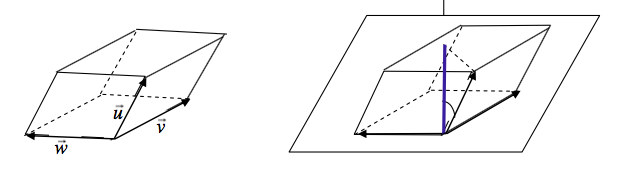
\includegraphics[height=3cm]{volum}
%\end{figure}


\end{document}